\section{Faisal Najib Abdullah(1174042)}
\subsection{Menginstalasi File Map Server}
Web Service yang digunakan pada map server ini adalah ms4w yang dapat didownload dari \href{https://ms4w.com/}{Link MS4W}.
Berikut cara untuk instalasinya : 
\begin{enumerate}
    \item Download file yang sudah berbentuk setub.exe lalu install next next saja
    \hfill\break
	\begin{figure}[H]
		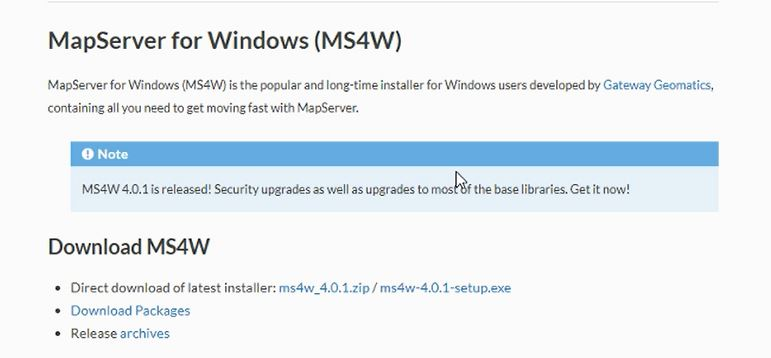
\includegraphics[width=8cm]{figures/1174042/T41.JPG}
		\centering
		\caption{Download File}
	\end{figure}
	
    \item Kemudian setelah menunggu lama kita di harus kan untuk menginstall Microsoft visual c lakukan install saja
    \hfill\break
	\begin{figure}[H]
		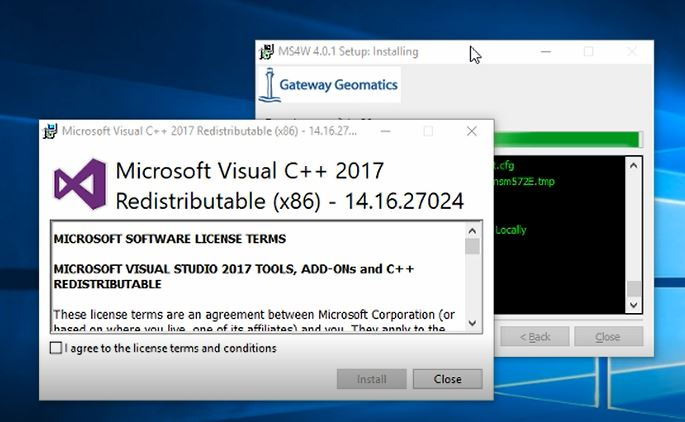
\includegraphics[width=8cm]{figures/1174042/T42.JPG}
		\centering
		\caption{Install Microsoft Visual C}
	\end{figure}
	
    \item kemudaian kita diminta untuk allow access Windows Security alert
    \hfill\break
	\begin{figure}[H]
		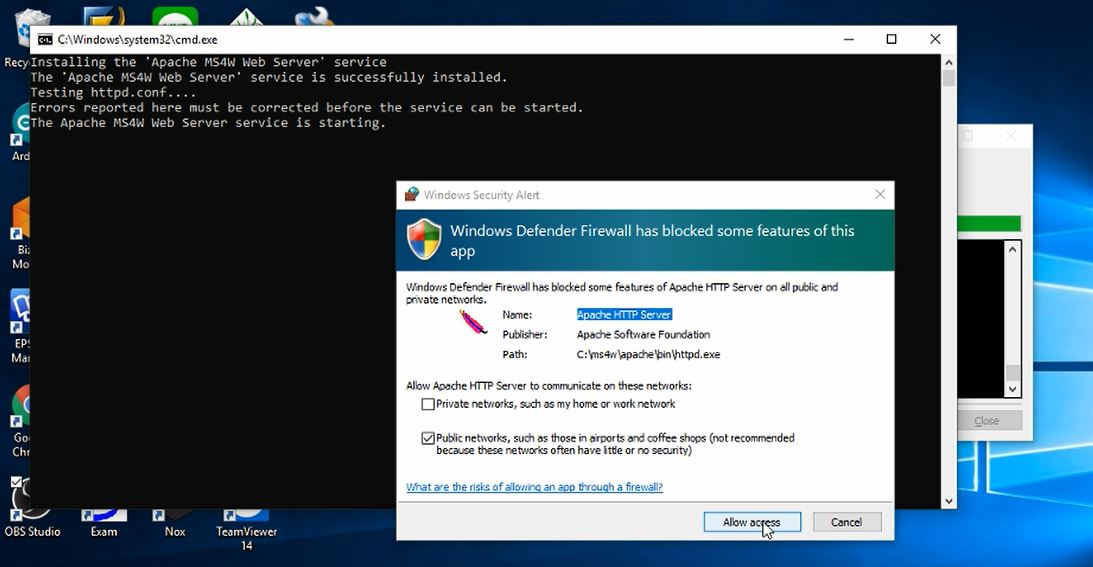
\includegraphics[width=8cm]{figures/1174042/T43.JPG}
		\centering
		\caption{Allow Access}
	\end{figure}
	
    \item Kemudian setelah selesai kita running pada directory tersebut dengan mapserv -v  
    \hfill\break
	\begin{figure}[H]
		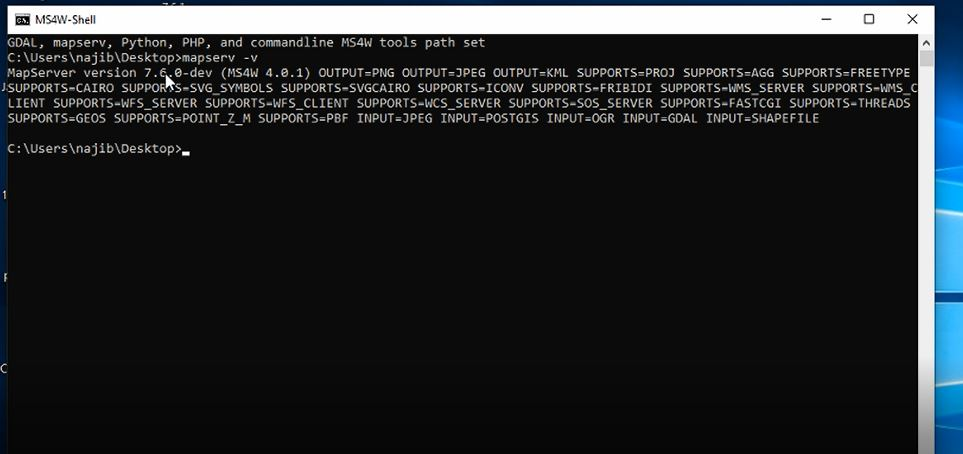
\includegraphics[width=8cm]{figures/1174042/T44.JPG}
		\centering
		\caption{Running}
	\end{figure}
	
    \item Kemudian setelah mapserver terinstall kita install mapproxy dengan cara pip install mapproxy
    \hfill\break
	\begin{figure}[H]
		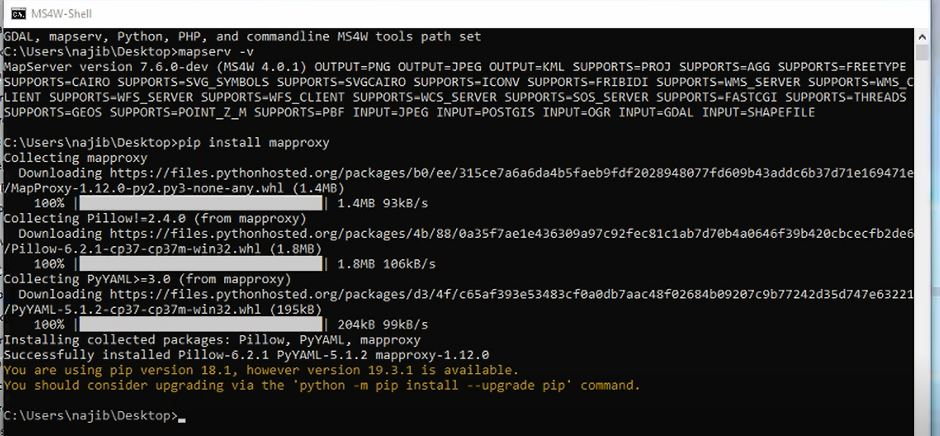
\includegraphics[width=8cm]{figures/1174042/T45.JPG}
		\centering
		\caption{Install Mapproxy}
	\end{figure}
\end{enumerate}

\subsection{Video Tutorial}
\href{https://www.youtube.com/watch?v=mYyPH4ofPxo}{Untuk Lebih jelasnya klik ini saja yah trimakasih}
